\documentclass[12pt,a4paper]{book}
\usepackage[minitoc]{teach}
\usepackage[utf8]{inputenc}
\usepackage[french]{babel}
\usepackage[T1]{fontenc}
\usepackage{amsmath}
\usepackage{amsfonts}
\usepackage{amssymb}
\usepackage{graphicx}
\renewcommand{\headrulewidth}{0pt}
\renewcommand{\footrulewidth}{0pt}
\fancyfoot[C]{\thepage}


\author{YAWO Kossi Atsu}
\newcommand{\prof}{YAWO Kossi Atsu}
\newcommand{\matiere}{MATHEMATIQUES}
\newcommand{\classe}{5$^{ème}$}
\title{Mes devoirs de Mathématiques}
\begin{document}
\begin{devoir}{DEVOIR SURVEILLE DU PREMIER TRIMESTRE}{\matiere}{\classe}{1}{1H 30}{13 novembre 2019}{\prof}
\begin{exo}[8]
\begin{multicols}{2}
Un trésor est caché dans le cour de l'école "LES MEILLEURS". Le plan ci-contre a été dressé par le fondateur et porte à son dos les renseignements suivants: "À égale distance du puits $(P)$ et de la cantine $(C)$, tu trouveras dans l'alignement du mât $(M_1)$ et du manguier $(M_2)$, enterrée à un profondeur de un (1) mètre, une caisse remplie de pierres précieuses."\\

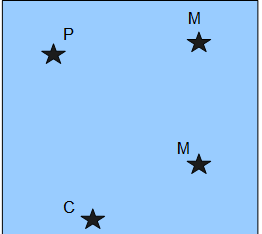
\includegraphics[scale=0.8]{images/dev120192020img1.png}
\end{multicols}

\vspace{0.5cm}
\underline{\textbf{Consignes}}\\
\begin{enumerate}
\item Reproduis ce plan.
\item Indique la position du trésor et explique ta méthode.
\end{enumerate}

\begin{tabular}{|c|c|c|c|c|}
\hline 
Critère & Pertinence & Correction & Cohérence & Perfectionnement \\ 
\hline
Barème & 2pts & 2pts & 3pts & 1pt \\ 
\hline 
\end{tabular}
\competence{•}{8}
\end{exo}

\begin{exo}[4]
\begin{defitemize}
\item Choisi la bonne réponse:
\begin{multicols}{2}
\begin{enumerate}
\item Si M est un point à l'intérieur du cercle $\mathcal{(C)}$ de centre A et de rayon 4cm, alors:
\begin{enumerate}
\item $AM=4cm$
\item $AM>4cm$
\item $AM<4cm$
\end{enumerate}
\item Si les points A, B et C du plan sont tels que $AB=7$, $BC=3cm$ et $AC=2,5$, alors:
\begin{enumerate}
\item A, B et C sont alignés
\item ABC est un triangle.
\item A, B et C ne forment pas un triangle.
\end{enumerate}
\item $(D)$ est la médiatrice du segment $[AB]$. Si $AM>BM$, alors:
\begin{enumerate}
\item Le point M appartient au demi-plan de frontière $(D)$ contenant le point A.
\item Le point M appartient au demi-plan de frontière $(D)$ contenant le point B.
\item Le point M appartient à $(D)$.
\end{enumerate}
\item La distance à zéro de (-13):
\begin{enumerate}
\item 13
\item -13
\item 1,3
\end{enumerate}
\end{enumerate}
\end{multicols}
\item réponds par vrai ou faux aux affirmations suivantes et corrige celle qui sont fausses:
\begin{enumerate}
\item L'ensemble des nombres entiers relatifs est noté: $\mathbb{Z}$.
\item Si deux nombres sont négatifs, alors le plus grand est celui qui a la plus grande valeur absolue.
\item Si deux nombres n'ont pas le même signe, alors le plus petit est le nombre négatif.
\end{enumerate}
\end{defitemize}

\end{exo}

\begin{exo}[8]
\begin{enumerate}
\item On donne les nombres suivants: $(-1)$ \qquad ; \qquad $(-13)$ \qquad ; \qquad $(0)$ \qquad ; \qquad $(+11)$ \qquad ; \qquad $(6,0)$
\begin{enumerate}
\item Parmi ces nombres, quels sont ceux qui: 
\begin{itemize}
\item sont positifs?
\item sont négatifs?
\item sont des entiers naturels?
\item sont des entiers relatifs?
\end{itemize} 
\item Donne l'opposé de chacun de ces nombres.
\item Range ces nombres dans l'ordre décroissant.
\end{enumerate}
\item Calcule les sommes suivantes:\\
$a=(-12)+(-8)$ \qquad ; \qquad $b=(-25)+(+30)$
\item Calcule les différences suivantes:\\
$c=(-9)-(-14)$ \qquad ; \qquad $d=(+25)-(+30)$
\item Calcule la sommes algébriques suivantes:\\
$a=(-12)-(-8)-(-25)+(-30)+(4)$
\item Sur une droite graduée, marque les points suivants: $A(-2)$ \qquad ;\qquad $B(3)$ \qquad ; \qquad $C(-3,5)$ \qquad ;\qquad $D(0)$.\\
Quelle est l'origine de cette droite graduée?
\end{enumerate}
\end{exo}
\end{devoir}

\newpage

\begin{td}{\matiere}{\classe}{23 novembre 2019}{\prof}
\begin{exo}
\begin{enumerate}
\item Complète chacune des phrases suivantes:
\begin{enumerate}
\item Deux angles sont \ldots lorsque la somme de leur mesures est $180\degres$
\item Deux angles sont \ldots lorsque la somme de leur mesures est $90\degres$
\item Dans un triangle, la \ldots des mesures des \ldots est $180\degres$.
\item Deux angles sont dits \ldots lorsque les côtés de l'un sont les \ldots aux côtés de l'autre.
\end{enumerate}
\item ABC est un triangle, complète le tableau suivant:\\
\begin{tabular}{|c|c|c|c|}
\hline 
$\widehat{A}$ & $30 \degres$ &  $25 \degres$ & • \\ 
\hline 
$\widehat{B}$ &  $60 \degres$ & • &  $48 \degres$ \\ 
\hline 
$\widehat{C}$ & • &  $52 \degres$ &  $72 \degres$ \\ 
\hline 
\end{tabular} 

\item $\widehat{P}$ et $\widehat{Q}$ sont des angles complémentaires; complète le tableau suivant:\\
\begin{tabular}{|c|c|c|c|}
\hline 
$\widehat{P}$ & $65 \degres$ &  $90 \degres$ & • \\ 
\hline 
$\widehat{Q}$ & • & • &  $1 \degres$ \\ 
\hline 
\end{tabular} 

\item $\widehat{M}$ et $\widehat{N}$ sont des angles supplémentaires; complète le tableau suivant:\\
\begin{tabular}{|c|c|c|c|}
\hline 
$\widehat{M}$ & $130 \degres$ &  $90 \degres$ & • \\ 
\hline 
$\widehat{N}$ & • & • &  $180 \degres$ \\ 
\hline 
\end{tabular} 

\item Réponds par vrai ou faux et corrige les affirmations fausses.
\begin{enumerate}
\item Si deux angles sont complémentaires, ils ne peuvent pas avoir la même mesure.
\item Deux angles sont supplémentaires, ils peuvent avoir la même mesure.
\item Si deux angles sont opposés par le sommet alors ils ont la même mesure.
\item Si deux angles sont complémentaires, alors aucun ne peut mesurer $90\degres$.
\end{enumerate}
\end{enumerate} 
\end{exo}

\vspace{0.5cm}

\begin{exo}
\begin{enumerate}
\item Calcule les sommes suivantes:\\
$E=(-5)+(-14)$ \qquad ; \qquad
$E=(+5,1)+(-7,4)$
\item Calcule les différences suivantes:\\
$E=(-5)-(+14)$ \qquad ; \qquad
$E=(-5,1)-(-7,4)$
\item Calcule les sommes algébriques suivantes:\\
$E=(-11)+(-19)-(-15)+(-5)-(-14)$ \qquad ; \qquad
$F=(-1,6)-(-3,9)-(+2,5)+(+5,1)-(+7,4)$
\end{enumerate}
\end{exo}

\vspace{0.5cm}
\begin{exo}
On donne les nombres décimaux suivants: $-4,2$ \qquad ; \qquad $3,2$ \qquad ; \qquad $-7$ \qquad ; \qquad $32$ \qquad ; \qquad $+12$\qquad et \qquad $0$
\begin{enumerate}
\item Parmi ces nombres, quels sont qui : 
\begin{enumerate}
\item sont positifs?
\item sont négatifs?
\item sont des nombres entiers naturels?
\item sont des nombres entiers relatifs?
\end{enumerate} 
\item Trouve l'opposé de chacun de ces nombres.
\item Range ces nombres par ordre croissant.
\end{enumerate}
\end{exo}
\end{td}

\begin{devoir}{COMPOSITION DU PREMIER TRIMESTRE}{\matiere}{\classe}{1}{1H 30}{13 décembre 2019}{\prof}

\begin{exo}[5]
\begin{multicols}{2}
Le mécanisme d'ouverture d'un coffre-fort est constitué de quatre cylindres sur chacun desquels sont inscrites les lettres de l'alphabet.
\begin{enumerate}
\item Combien de combien de codes est-il possible de former?
\item Kodjovi, un petit matheux affirme qu'il faudra plus d'un mois(jours et nuits) à des cambrioleurs, pour parvenir à essayer tous ces codes s'ils essaye un code tous les 6 minuites. As-t-il raison?
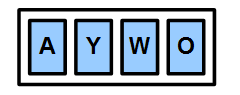
\includegraphics[scale=0.8]{images/compo1img1.png}
\end{enumerate}
\end{multicols}
\competence{•}{5}
\end{exo}

\vspace{0.5cm}

\begin{exo}[5]
\begin{multicols}{2}
\begin{enumerate}
\item Complète chacune des phrases suivantes:
\begin{enumerate}
\item Deux angles sont \ldots lorsque la somme de leur mesures est $180\degres$
\item Deux angles sont \ldots lorsque la somme de leur mesures est $90\degres$
\item Dans un triangle, la \ldots des mesures des \ldots est $180\degres$.
\item Deux angles sont dits \ldots lorsque les côtés de l'un sont les \ldots aux côtés de l'autre.
\end{enumerate}
\item ABC est un triangle, complète le tableau suivant:\\
\begin{tabular}{|c|c|c|c|}
\hline 
$\widehat{A}$ & $30 \degres$ &  $25 \degres$ & • \\ 
\hline 
$\widehat{B}$ &  $60 \degres$ & • &  $48 \degres$ \\ 
\hline 
$\widehat{C}$ & • &  $52 \degres$ &  $72 \degres$ \\ 
\hline 
\end{tabular} 

\item $\widehat{P}$ et $\widehat{Q}$ sont des angles complémentaires; complète le tableau suivant:\\
\begin{tabular}{|c|c|c|c|}
\hline 
$\widehat{P}$ & $65 \degres$ &  $90 \degres$ & • \\ 
\hline 
$\widehat{Q}$ & • & • &  $1 \degres$ \\ 
\hline 
\end{tabular} 

\item $\widehat{M}$ et $\widehat{N}$ sont des angles supplémentaires; complète le tableau suivant:\\
\begin{tabular}{|c|c|c|c|}
\hline 
$\widehat{M}$ & $130 \degres$ &  $90 \degres$ & • \\ 
\hline 
$\widehat{N}$ & • & • &  $180 \degres$ \\ 
\hline 
\end{tabular} 

\item Réponds par vrai ou faux et corrige les affirmations fausses.
\begin{enumerate}
\item Si deux angles sont complémentaires, ils ne peuvent pas avoir la même mesure.
\item Deux angles sont supplémentaires, ils peuvent avoir la même mesure.
\item Si deux angles sont opposés par le sommet alors ils ont la même mesure.
\item Si deux angles sont complémentaires, alors aucun ne peut mesurer $90\degres$.
\end{enumerate}
\end{enumerate} 
\end{multicols}
\competence{•}{5}
\end{exo}

\vspace{0.5cm}

\begin{exo}[7,5]
\begin{multicols}{2}
\begin{enumerate}
\item Calcule les sommes suivantes:\\
$E=(-5)+(-14)$ \qquad ; \qquad
$F=(+5,1)+(-7,4)$
\item Calcule les différences suivantes:\\
$G=(-5)-(+14)$ \qquad ; \qquad
$H=(-5,1)-(-7,4)$
\item Calcule les sommes algébriques suivantes:\\
$I=(-11)+(-19)-(-15)+(-5)-(-14)$ \qquad ; \qquad\\
$J=(-1,6)-(-3,9)-(+2,5)+(+5,1)-(+7,4)$

\item On donne les nombres décimaux suivants: $-4,2$ \qquad ; \qquad $3,2$ \qquad ; \qquad $-7$ \qquad ; \qquad $32$ \qquad ; \qquad $+12$\qquad et \qquad $0$
\item Parmi ces nombres, quels sont qui : 
\begin{enumerate}
\item sont positifs?
\item sont négatifs?
\item sont des nombres entiers naturels?
\item sont des nombres entiers relatifs?
\end{enumerate} 
\item Trouve l'opposé de chacun de ces nombres.
\item Range ces nombres par ordre croissant.
\end{enumerate}
\end{multicols}
\competence{}{7.5}
\end{exo}

\vspace{0.5cm}
\begin{exo}[2.5]
Écris sous la forme d'une puissance d'un nombre entier relatif:\\
$k=25\times125$ \qquad; \qquad $l=3\times3\time27\times9$ \qquad; \qquad $m=9^7\times9^{12}$ \qquad; \qquad $n=5^3\times1^{10}$ \qquad; \qquad $o=3^5\times4^5$
\competence{•}{3}
\end{exo}

\tableofcompetences
\end{devoir}

\newpage
\begin{td}{\matiere}{\classe}{$1^{er}$ février 2020}{\prof}
\begin{exo}
Reproduis la figure ci-contre. Le point A est son propre symétrique par rapport à une droite $(L)$ qui a été effacée. Le symétrique $C'$ du point $C$ par rapport à $(L)$ appartient à la droite  $(D)$.
\begin{enumerate}
\item Donne un programme de construction de la droite $(L)$. 
\item Construis la droite $(L)$.
\item Construis le symétrique $A'B'C'$ du triangle $ABC$ par rapport à $(L)$.
\item Compare les mesures des angles des triangles $ABC$ et $A'B'C'$. Justifie ta réponse.
\end{enumerate}
\end{exo}

\vspace{1cm}
\begin{exo}
\begin{enumerate}
\item Pour chaque ligne, indiquer la ou les bonne réponses:\\
\begin{tabular}{|c|c|c|c|c|}
\hline 
N° & Question & Réponse A & Réponse B & Réponse C \\ 
\hline 
1 & 3 exposant 4 s'écrit & $3 \times 4$ & $3^4$& $4^3$\\ 
\hline 
2 & $5\times5\times5\times5\times5\times5$ & $5^6$ & $6^5$ &$5^5$\\ 
\hline 
3 & $2^6$ & $32$ & $64$ &$12$ \\ 
\hline
4 & $(-1)^6$ & $1$ & $-1$ &$6$ \\ 
\hline
5 & $1^100$ & $1$ & $0$ &$100$ \\ 
\hline
6 & $2,5^2$ & $5$ & $6,25$ &$5,65$ \\ 
\hline
\end{tabular} 

\item Reproduis puis complète le tableau suivant:\\
\begin{tabular}{|c|c|c|c|c|}
\hline 
Règle & $a^m\times a^n=\ldots$ & $(a\times b)^n=\ldots$\\ 
\hline 
1 & $3^4 \times 3^5=\ldots$ & $(2\times 3)^4=\ldots$\\ 
\hline 
2 & $4^{\ldots} \times 4^5=4^8$ & $(2\times \ldots)^4=10^4$\\ 
\hline 
3 & $\ldots^2 \times \ldots^5=2^7$ & $(7\times 4)^4=\ldots^4$\\ 
\hline 
\end{tabular} 

\item Reproduis puis mets une croix dans la case qui convient:\\
\begin{tabular}{|c|c|c|c|c|}
\hline 
 & Vrai & Faux\\ 
\hline 
$2\times 2+3\times 3=2^2+3^3$ &  & \\ 
\hline 
$(3+4)^2=3^2+4^2$ &  & \\ 
\hline
$(3\times 4)^2=3^2+4^2$ &  & \\ 
\hline
$5^2\times 4^3=(5\times 4)^2\times 4$ &  & \\ 
\hline
$3^2\times 9\times 5^4=(3\times 5)^4$ &  & \\ 
\hline
$27 \times 25=(5\times 3)^2$ &  & \\ 
\hline
\end{tabular} 
\end{enumerate}
\end{exo}

\begin{exo}
\begin{enumerate}
\item On donne $a=(-2,7)$, $b=(+6,5)$ et $c=(+3,1)$. Calcule:
\begin{enumerate}
\item $a-b$
\item $a+b-c$
\item $a-opp(b)+opp(opp(c))$
\end{enumerate}
\item Résoudre les équations suivantes:
$x+(+3)=(+5)$ \qquad et \qquad $ x+(-8)=(-5)$
\end{enumerate}
\end{exo}

\end{td}


\newpage
\begin{devoir}{DEVOIR SURVEILLÉ DU DEUXIÈME TRIMESTRE}{\matiere}{\classe}{2}{1H 30'}{12 février 2020}{\prof}
\begin{exo}[6]
Reproduis la figure ci-contre. Le point A est son propre symétrique par rapport à une droite $(L)$ qui a été effacée. Le symétrique $C'$ du point $C$ par rapport à $(L)$ appartient à la droite  $(D)$.
\begin{enumerate}
\item Donne un programme de construction de la droite $(L)$. 
\item Construis la droite $(L)$.
\item Construis le symétrique $A'B'C'$ du triangle $ABC$ par rapport à $(L)$.
\item Compare les mesures des angles des triangles $ABC$ et $A'B'C'$. Justifie ta réponse.
\end{enumerate}
\end{exo}

\begin{exo}[10]
\begin{enumerate}
\item Pour chaque ligne, indiquer la ou les bonne réponses:\\
\begin{tabular}{|c|c|c|c|c|}
\hline 
N° & Question & Réponse A & Réponse B & Réponse C \\ 
\hline 
1 & 3 exposant 4 s'écrit & $3 \times 4$ & $3^4$& $4^3$\\ 
\hline 
2 & $5\times5\times5\times5\times5\times5$ & $5^6$ & $6^5$ &$5^5$\\ 
\hline 
3 & $2^6$ & $32$ & $64$ &$12$ \\ 
\hline
4 & $(-1)^6$ & $1$ & $-1$ &$6$ \\ 
\hline
5 & $1^100$ & $1$ & $0$ &$100$ \\ 
\hline
6 & $2,5^2$ & $5$ & $6,25$ &$5,65$ \\ 
\hline
\end{tabular} 

\item Reproduis puis mets une croix dans la case qui convient:\\
\begin{tabular}{|c|c|c|c|c|}
\hline 
 & Vrai & Faux\\ 
\hline 
$2\times 2+3\times 3=2^2+3^3$ &  & \\ 
\hline 
$(3+4)^2=3^2+4^2$ &  & \\ 
\hline
$(3\times 4)^2=3^2+4^2$ &  & \\ 
\hline
$5^2\times 4^3=(5\times 4)^2\times 4$ &  & \\ 
\hline
$3^2\times 9\times 5^4=(3\times 5)^4$ &  & \\ 
\hline
$27 \times 25=(5\times 3)^2$ &  & \\ 
\hline
\end{tabular} 
\item On donne $a=(-2,7)$, $b=(+6,5)$ et $c=(+3,1)$. \\
Calcule:
$\textbf{a-b}$ \qquad ;\qquad $\textbf{a+b-c}$ \qquad et \qquad $\textbf{a-opp(b)+opp(opp(c))}$

\item Résoudre les équations suivantes:
$x+(+3)=(+5)$ \qquad et \qquad $x+(-8)=(-5)$
\item Dans chacun des cas suivants, complète par le nombre entier naturel qui convient:\\
$17 \times \ldots=255$ \qquad ;\qquad $\ldots \times 13=143$ \qquad ;\qquad $5436=\ldots \times 16 +12$.
\end{enumerate}
\end{exo}

\begin{exo}[4]
Dans chacun des cas de figures ci-dessous, détermine la mesure de l'angle indiqué par le point d'interrogation (?). Justifie tes réponses.\\
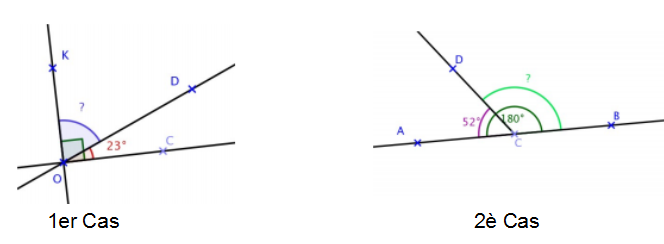
\includegraphics[scale=0.7]{images/dev2_2020_img1.png}
\end{exo}

\end{devoir}

\begin{td}{\matiere}{\classe}{29 février 2020}{\prof}
\begin{exo}
À la fin d'une fête de village, tous les enfants présents se partagent équitablement les 397 ballons de baudruche qui ont servi à la décoration. Il reste alors 37 ballons. L'année suivante, les mêmes enfants se partagent les 598 ballons utilisés cette années-là. Il en reste alors 13. \\
Combien d'enfants, au maximum, étaient présents?
\end{exo}

\begin{exo}
Une commerçante reçoit 700 sucettes acidulées: 390 sont au goût pomme; les sucettes restantes son au goût orange. Elle souhaite réaliser des sachets identiques avec un assortiment des deux types de sucettes, de façon à ce que tout son stock soit utilisé.\\
Indique toutes les possibilités. Préciser, pour chaque cas, la composition des sachets.
\end{exo}

\begin{exo}
\setlength{\columnseprule}{1pt}
\begin{multicols}{2}
Indique si les phrases suivantes sont vraies ou fausses et justifie.
\begin{enumerate}
\item Si un nombre est premier alors ne peut être pair.
\item Tous les nombres pairs plus grands que 2 ne sont pas premiers.
\item Tous les nombres premiers sont impairs.
\item Tous les nombres impairs sont premiers.
\item La différences entre deux nombres premiers successifs est deux.
\item 57 est un nombre premier.
\item Si un nombre est compris entre $5 \times 11$ et $5 \times 12$, alors le quotient de la division euclidienne de ce nombre par 5 est égal à 11.
\item Si le quotient de la division euclidienne d'un nombre par 9 est égal à 60, alors ce nombre est égal à $60 \times 9$.
\end{enumerate}
\end{multicols}

\end{exo}

\begin{exo}
\setlength{\columnseprule}{1pt}
\begin{multicols}{2}
Les points B, A et C sont alignés.\\
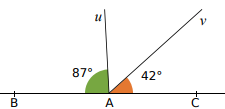
\includegraphics[scale=0.9]{images/td_29_02_2020_img1.png}\\
Calcule, en détaillant, la mesure des angles :
$\widehat{uAv}$ \qquad ;\qquad $\widehat{BAv}$ et $\widehat{uAC}$
\end{multicols}

\end{exo}

\begin{exo}
\setlength{\columnseprule}{1pt}
\begin{multicols}{2}
Sur la figure ci-dessous, les points O, A et L sont alignés.\\
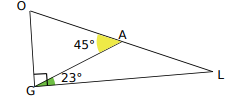
\includegraphics[scale=0.9]{images/td_29_02_2020_img2.png}\\

\begin{enumerate}
\item Quelle est la mesure et la nature de l'angle  $\widehat{OGA}$ ? Justifie.
\item Quelle est la mesure et la nature de l'angle  $\widehat{GAL}$ ? Justifie.
\end{enumerate}

\end{multicols}
\end{exo}

\begin{exo}
\setlength{\columnseprule}{1pt}
\begin{multicols}{2}
\begin{enumerate}
\item Construis un triangle ACD tel que : $DC = 6 cm$ ; $\widehat{CDA}= 67 \degres$ et $\widehat{DCA} = 36 \degres$.
\item À l'extérieur du triangle ADC, construis le point B tel que $CAB = 58\degres$ et $AB = 8,2 cm$ puis trace le segment [BC]. 
\item Quelle est la nature des angles $\widehat{DAB}$, $\widehat{DCB}$ et $\widehat{ABC}$ ?
\end{enumerate}
\end{multicols}
\end{exo}

\end{td}

\begin{devoir}{COMPOSITION DU DEUXIÈME TRIMESTRE}{\matiere}{\classe}{1}{1H 30}{11 mars 2020}{\prof}

\begin{exo}[5]
Une commerçante reçoit 700 sucettes acidulées: 390 sont au goût pomme; les sucettes restantes son au goût orange. Elle souhaite réaliser des sachets identiques avec un assortiment des deux types de sucettes, de façon à ce que tout son stock soit utilisé.\\
Indique toutes les possibilités. Préciser, pour chaque cas, la composition des sachets.
\end{exo}

\vspace{0.5cm}

\begin{exo}[10]
\setlength{\columnseprule}{1pt}
\begin{enumerate}
\item Indique si les phrases suivantes sont vraies ou fausses et justifie.
\begin{multicols}{2}
\begin{enumerate}
\item Si un nombre est premier alors ne peut être pair.
\item Tous les nombres pairs plus grands que 2 ne sont pas premiers.
\item Tous les nombres premiers sont impairs.
\item Tous les nombres impairs sont premiers.
\item 1 est un nombre premier.
\item 8 est un nombre premier.
\end{enumerate}
\end{multicols}
\item Cite les nombres premiers compris entre 0 et 20.
\item \begin{enumerate}
\item Décompose chacun des nombres suivants en produit de facteurs premiers: \\
 20 \qquad ;  \qquad 12 \qquad ;  \qquad 18 \qquad et  \qquad 36. 
\item Utilise les décompositions précédentes pour calculer:\\
$PPCM(18 ; 20)$ et $PPCM(12 ; 20)$
\item Rends irréductible chacune des fractions suivantes:\\
$\frac{18}{36}$ \qquad ; \qquad $\frac{20}{18}$
\item Déduis-en $PGCD(18;36)$ \qquad et \qquad $PGCD(18;20)$
\end{enumerate}
\item Effectue les calculs suivants:\\
$A=\frac{7}{5}-\frac{3}{5}$ \qquad ; \qquad $B=\frac{4}{13}+\frac{3}{13}$ \qquad ; \qquad $C=\frac{7}{10}+\frac{11}{15}$ \qquad et \qquad $D=\frac{7}{20}-\frac{3}{5}+\frac{7}{10}$
\end{enumerate}
\end{exo}

\vspace{0.5cm}

\begin{exo}[5]
\setlength{\columnseprule}{1pt}

\begin{enumerate}
\item \begin{multicols}{2}
Sur la figure ci-contre, les points B, A et C sont alignés.\\
Calcule, en détaillant, la mesure des angles :
$\widehat{uAv}$ \qquad ;\qquad $\widehat{BAv}$ et $\widehat{uAC}$\\
\begin{center}
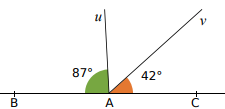
\includegraphics[scale=0.9]{images/td_29_02_2020_img1.png}
\end{center}
\end{multicols}

\item \begin{multicols}{2}
Sur la figure ci-dessous, les points O, A et L sont alignés.
\begin{enumerate}
\item Quelle est la mesure et la nature de l'angle  $\widehat{OGA}$ ? Justifie.
\item Quelle est la mesure et la nature de l'angle  $\widehat{GAL}$ ? Justifie.
\end{enumerate}

\begin{center}
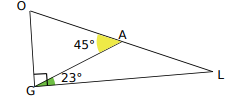
\includegraphics[scale=0.9]{images/td_29_02_2020_img2.png}\\
\end{center}
\end{multicols}
\end{enumerate}

\end{exo}

\end{devoir}
\end{document}
